% !TEX root = ../main.tex

\section{Cograph definitions}

Cographs can be defined in several equivalent ways. This paper will provide four different definitions and proofs that these definitions are equivalent. Some other definitions of cographs (there referred to as hereditary Dacey graphs or HD-graphs) and their properties can be found in \cite{sumner}.

\begin{defi}\label{codef1}
    Let us define set of graphs $\Cographs$ as the smallest set that satisfies:
    \begin{enumerate}
        \item $\forall_v \singleton{v} \in \Cographs$
        \item $\forall_G \Gcomp{G} \in \Cographs$
        \item $\forall_{G_1, G_2} \V(G_1) \cap \V(G_2) \implies \Gunion{G_1}{G_2} \in \Cographs$
    \end{enumerate}
    Graph $G$ is a \emph{cograph} if and only if $G \in \Cographs$.
\end{defi}
\begin{defi}\label{codef2}
    Let us define set of graphs $\Cographs$ as the smallest set that satisfies:
    \begin{enumerate}
        \item $\forall_v \singleton{v} \in \Cographs$
        \item $\forall_{G_1, G_2} \V(G_1) \cap \V(G_2) \implies \Gjoin{G_1}{G_2} \in \Cographs$
        \item $\forall_{G_1, G_2} \V(G_1) \cap \V(G_2) \implies \Gunion{G_1}{G_2} \in \Cographs$
    \end{enumerate}
    Graph $G$ is a \emph{cograph} if and only if $G \in \Cographs$.
\end{defi}

\begin{defi}
    \emph{Cotree} $C$ is a tuple $(T, \kind)$ where $T$ is a tree and $\kind$ is a function $\V(T) \to \{s,0,1\}$ such that for each $t \in \V(T)$ it satisfies:
    \begin{enumerate}
        \item $\kind(\R(T)) = 1$
        \item $\kind(t) = s \implies \C(t) = \emptyset$.
        \item $\kind(t) = 0 \implies \C(t) \neq \emptyset \land \forall_{t' \in \C(t)} \kind(t') \neq 0$.
        \item $\kind(t) = 1 \implies \C(t) \neq \emptyset \land \forall_{t' \in \C(t)} \kind(t') \neq 1$.
    \end{enumerate}
\end{defi}

\begin{defi}\label{codef3}
    Let $(T, \kind)$ be a cotree and let $L = \{v : v \in \V(T) \land \kind(v) = s\}$. \emph{Cograph defined by cotree $T$} denoted $\G(T)$ is a graph $(L, \{\{u,v\} : \{u,v\} \in L \land \kind(\LCA_T(u,v)\}) = 1)$.

    Graph $G$ is a \emph{cograph} if and only if there exists cotree $T$ such that $G = \G(T)$.
\end{defi}

\begin{figure}[h]
    \centering
    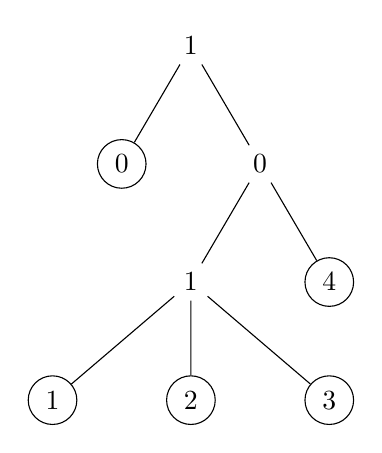
\begin{tikzpicture}[leaf/.style = {circle, draw}, sibling distance=5em]
        \node {1}
        child { node[leaf] {0} }
        child { node {0}
                child { node {1}
                        child { node[leaf] {1} }
                        child { node[leaf] {2} }
                        child { node[leaf] {3} } }
                child { node[leaf] {4} } };
    \end{tikzpicture}\hspace{5em}
    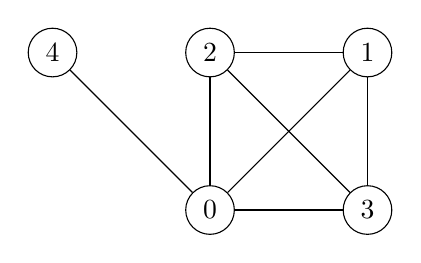
\begin{tikzpicture}
        \begin{scope}[every node/.style={draw, circle}]
            \node (0) at (0,0) {0};
            \node (1) at (2,2) {1};
            \node (2) at (0,2) {2};
            \node (3) at (2,0) {3};
            \node (4) at (-2,2) {4};
        \end{scope}

        \begin{scope}[
                every edge/.style={draw}]
            \path [-] (1) edge (2);
            \path [-] (2) edge (3);
            \path [-] (3) edge (1);
            \path [-] (0) edge (1);
            \path [-] (0) edge (2);
            \path [-] (0) edge (3);
            \path [-] (0) edge (4);
        \end{scope}
    \end{tikzpicture}
    \caption{A cotree (left) and cograph defined by it (right). Formally the pictured cotree would be written as $T = ((V, p), \kind)$, where $V = \{0, \ldots, 7\}$, $p = \{(0, 7), (1,5), (2,5), (3,5), (4,6), (5,6), (6,7), (7,\bot)\}$ and $\kind =\{(0,s), (1,s), (2,s), (3,s), (4,s), (5,1), (6,0), (7,1)\}$}
\end{figure}

\begin{defi}\label{codef4}
    Graph $G$ is a \emph{cograph} if and only if for each $X \subseteq \V(G)$ graphs $G[X]$ and $P_4 = (\{0,1,2,3\}, \{\{0,1\},\{1,2\},\{2,3\}\})$ are non-isomorphic.
\end{defi}

\begin{defi}\label{codef5}
    Graph $G$ is a \emph{cograph} if and only if either $G = \singleton{v}$ for $v \in \Vertices$ or for each $X \subseteq \V(G)$ either $G[X]$ is disconnected or $\Gcomp{G[X]}$ is disconnected.
\end{defi}
